\documentclass[tikz,border=10pt]{standalone}
\usetikzlibrary{positioning, arrows.meta, calc, babel, fit}
\usepackage[utf8]{inputenc}
\usepackage[T1]{fontenc}
\usepackage{lmodern}
\usepackage[english]{babel}
\usepackage{amsmath, amssymb, bm}

\begin{document}
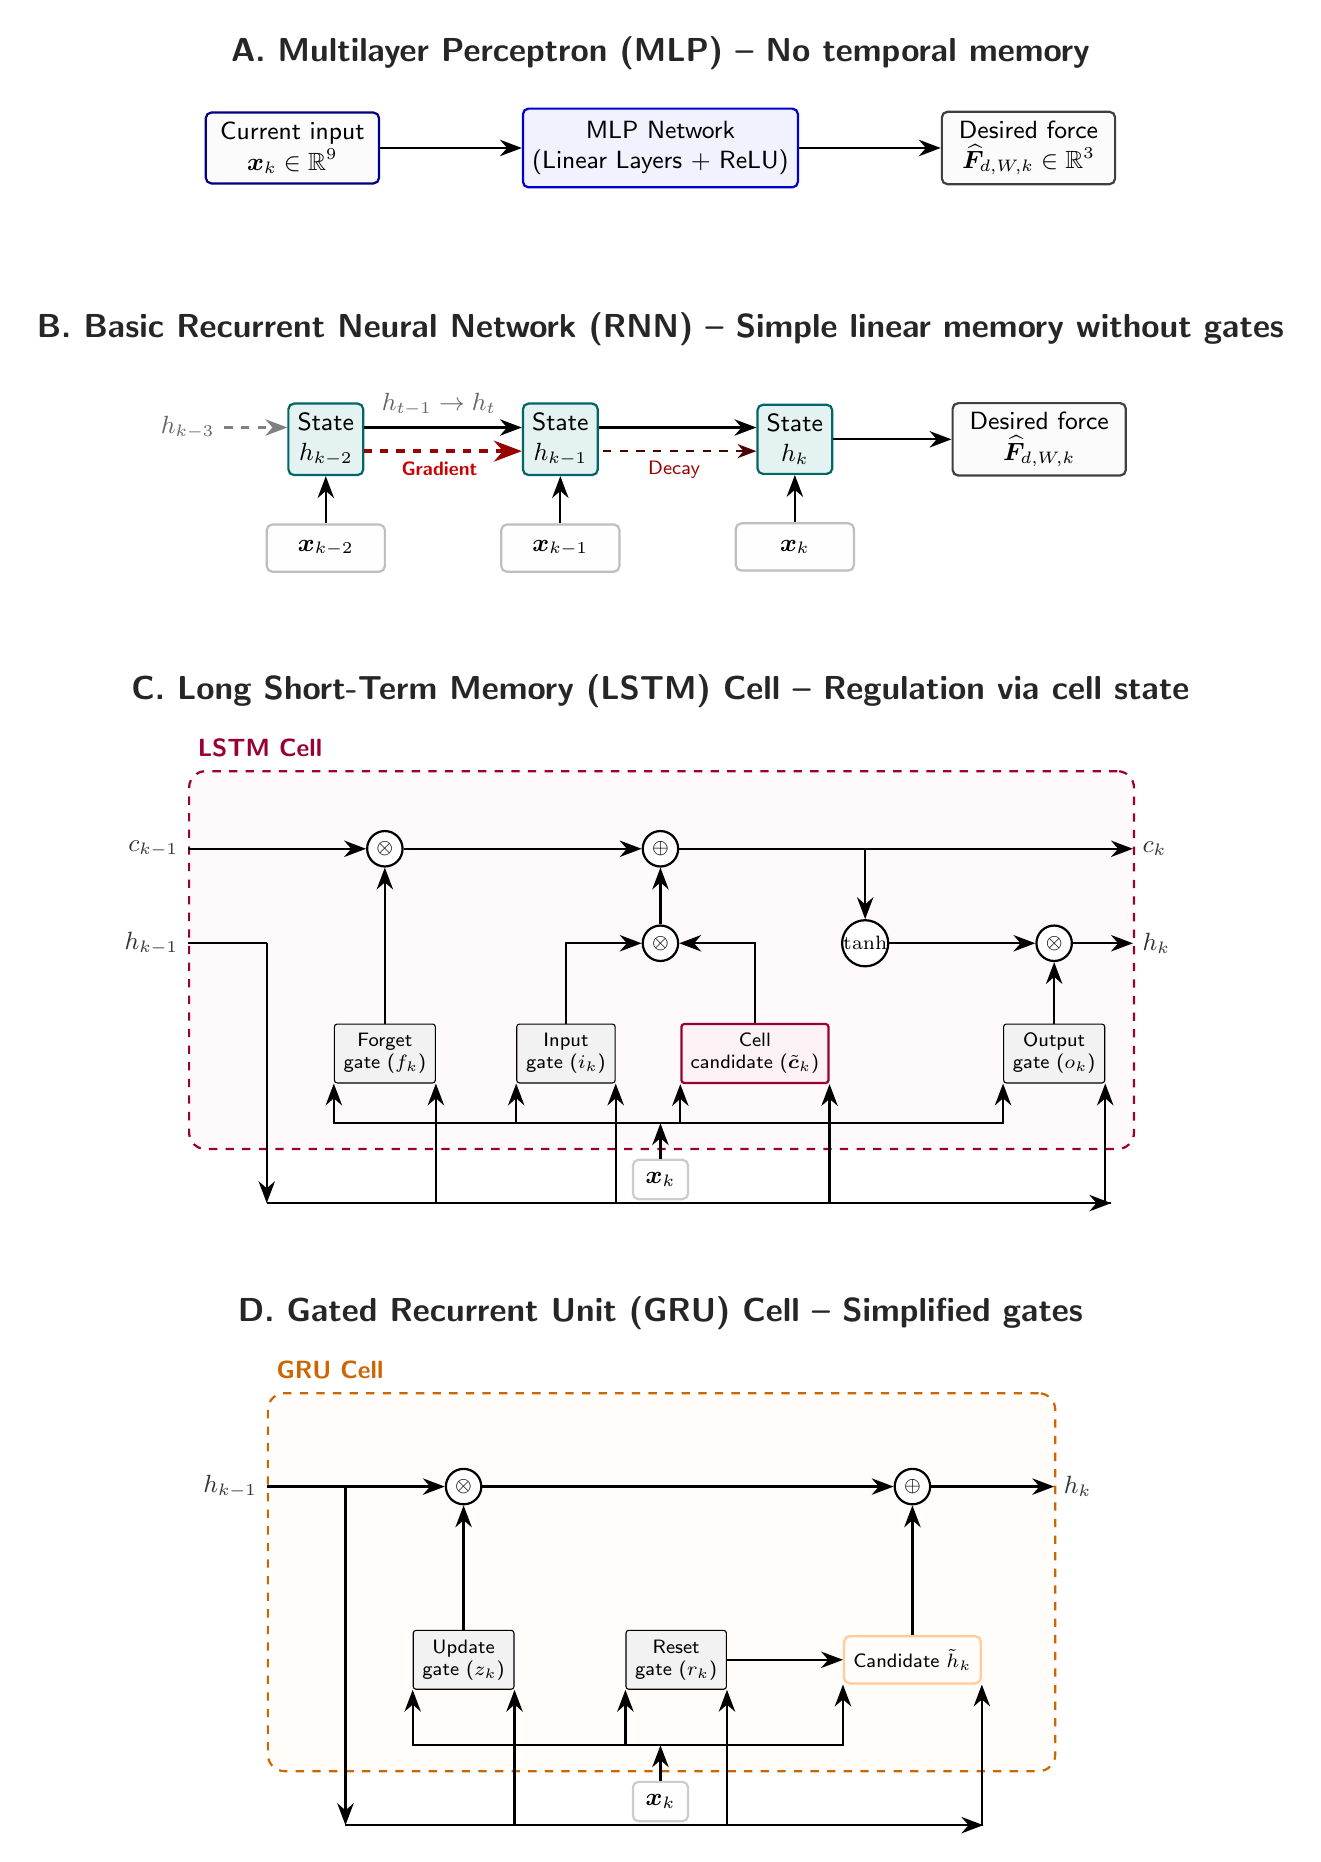
\begin{tikzpicture}[
  node distance=0.6cm and 0.8cm,
  align=center,
  font=\sffamily\small,
  % Estilos de bloques principales
  box/.style={draw, rectangle, rounded corners=2pt, minimum width=2.2cm, minimum height=0.9cm, thick, fill=white},
  mlpbox/.style={draw=blue!80!black, rectangle, rounded corners=2pt, minimum width=3.2cm, minimum height=1.0cm, thick, fill=blue!5},
  rnnbox/.style={draw=teal!80!black, rectangle, rounded corners=2pt, minimum size=0.8cm, thick, fill=teal!10},
  cellbox/.style={draw=purple!80!black, rectangle, rounded corners=6pt, dashed, thick, fill=purple!2},
  grubox/.style={draw=orange!80!black, rectangle, rounded corners=6pt, dashed, thick, fill=orange!2},
  % Operaciones matemáticas internas
  op/.style={draw, circle, minimum size=0.45cm, inner sep=0pt, thick, fill=white, font=\sffamily\scriptsize},
  gate/.style={draw, rectangle, rounded corners=1pt, minimum width=1.25cm, minimum height=0.65cm, fill=gray!10, font=\sffamily\scriptsize},
  % Estilos de flechas
  line/.style={draw, -{Stealth[scale=1.2]}, thick},
  gradline/.style={draw, {Stealth[scale=1.2]}-, dashed, red!80!black, thick},
  labeltext/.style={font=\sffamily\small, text=black!80}
]

  % ==========================================
  % PANEL A: FEEDFORWARD CASE (MLP) - NO MEMORY
  % ==========================================
  \node[font=\sffamily\bfseries\large, text=black!85, anchor=center] (tituloA) at (11.2, 8.5) {A. Multilayer Perceptron (MLP) -- No temporal memory};
  
  \node[mlpbox] (nnA) at (11.2, 7.3) {MLP Network\\(Linear Layers + ReLU)};
  \node[box, draw=blue!50!black, fill=gray!3, left=1.8cm of nnA] (inputA) {Current input\\$\bm{x}_k \in \mathbb{R}^9$};
  \node[box, draw=gray!50!black, fill=gray!3, right=1.8cm of nnA] (outputA) {Desired force\\$\widehat{\bm{F}}_{d,W,k} \in \mathbb{R}^3$};

  \draw[line] (inputA) -- (nnA);
  \draw[line] (nnA) -- (outputA);

  % ==========================================
  % PANEL B: BASIC RECURRENT NETWORK (RNN) - SIMPLE MEMORY
  % ==========================================
  \node[font=\sffamily\bfseries\large, text=black!85, anchor=center] (tituloB) at (11.2, 5.0) {B. Basic Recurrent Neural Network (RNN) -- Simple linear memory without gates};

  % Desenrollado temporal k-2, k-1, k
  \node[rnnbox] (h0) at (6.95, 3.6) {State\\$h_{k-2}$};
  \node[rnnbox, right=2.0cm of h0] (h1) {State\\$h_{k-1}$};
  \node[rnnbox, right=2.0cm of h1] (h2) {State\\$h_{k}$};
  
  \node[box, draw=gray!50, fill=gray!1, minimum width=1.5cm, minimum height=0.6cm, below=0.6cm of h0] (x0) {$\bm{x}_{k-2}$};
  \node[box, draw=gray!50, fill=gray!1, minimum width=1.5cm, minimum height=0.6cm, below=0.6cm of h1] (x1) {$\bm{x}_{k-1}$};
  \node[box, draw=gray!50, fill=gray!1, minimum width=1.5cm, minimum height=0.6cm, below=0.6cm of h2] (x2) {$\bm{x}_{k}$};

  \node[box, draw=gray!50!black, fill=gray!3, right=1.5cm of h2] (outputB) {Desired force\\$\widehat{\bm{F}}_{d,W,k}$};

  % Conexiones verticales
  \draw[line] (x0) -- (h0);
  \draw[line] (x1) -- (h1);
  \draw[line] (x2) -- (h2);

  % Conexiones horizontales (paso del tiempo)
  \draw[line] ($(h0.east) + (0,0.15)$) -- node[above=0.02cm, font=\sffamily\small, text=black!60] {$h_{t-1} \to h_t$} ($(h1.west) + (0,0.15)$);
  \draw[line] ($(h1.east) + (0,0.15)$) -- ($(h2.west) + (0,0.15)$);
  \draw[line] (h2) -- (outputB);
  
  % Conexiones del gradiente (retropropagación hacia atrás)
  \draw[gradline, red!60!black, line width=1.2pt] ($(h1.west) + (0,-0.15)$) -- node[below, font=\sffamily\scriptsize\bfseries, text=red!80!black] {Gradient} ($(h0.east) + (0,-0.15)$);
  \draw[gradline, red!30!black, line width=0.6pt] ($(h2.west) + (0,-0.15)$) -- node[below, font=\sffamily\scriptsize, text=red!60!black] {Decay} ($(h1.east) + (0,-0.15)$);
  
  % Entrada y salida del flujo temporal general
  \draw[line, dashed, gray] ($(h0.west) + (-0.8,0.15)$) -- ($(h0.west) + (0,0.15)$);
  \node[left=0.8cm of h0, yshift=0.15cm, font=\sffamily\small, text=black!60] {$h_{k-3}$};

  % ==========================================
  % PANEL C: LONG SHORT-TERM MEMORY (LSTM) CELL
  % ==========================================
  \node[font=\sffamily\bfseries\large, text=black!85, anchor=center] (tituloC) at (11.2, 0.4) {C. Long Short-Term Memory (LSTM) Cell -- Regulation via cell state};

  \coordinate (lstmorigen) at (5.2, -0.6);

  \node[cellbox, minimum width=12.0cm, minimum height=4.8cm, anchor=north west] (lstmcella) at (lstmorigen) {};
  \node[above=0.05cm of lstmcella.north west, anchor=south west, font=\sffamily\bfseries\small, text=purple!80!black] {LSTM Cell};

  % Carril superior: estado de celda c_k
  \node[labeltext, anchor=east] (c_prev) at ($(lstmorigen) + (0, -1.0)$) {$c_{k-1}$};
  \node[op] (mult_f) at ($(lstmorigen) + (2.5, -1.0)$) {$\otimes$};
  \node[op] (add_i) at ($(lstmorigen) + (6.0, -1.0)$) {$\oplus$};
  \node[labeltext, anchor=west] (c_next) at ($(lstmorigen) + (12.0, -1.0)$) {$c_k$};

  % Fila de compuertas y candidato (columnas alineadas con operaciones)
  \node[gate] (gate_f) at ($(lstmorigen) + (2.5, -3.6)$) {Forget\\gate ($f_k$)};
  \node[gate] (gate_i) at ($(lstmorigen) + (4.8, -3.6)$) {Input\\gate ($i_k$)};
  \node[gate, draw=purple!80!black, fill=purple!5, thick] (gate_c) at ($(lstmorigen) + (7.2, -3.6)$) {Cell\\candidate ($\tilde{\bm{c}}_k$)};
  \node[gate] (gate_o) at ($(lstmorigen) + (11.0, -3.6)$) {Output\\gate ($o_k$)};

  % Carril de salida oculta (operaciones intermedias)
  \node[labeltext, anchor=east] (h_prev) at ($(lstmorigen) + (0, -2.2)$) {$h_{k-1}$};
  \node[op] (mult_i) at ($(lstmorigen) + (6.0, -2.2)$) {$\otimes$};
  \node[op] (tanh_act) at ($(lstmorigen) + (8.6, -2.2)$) {$\tanh$};
  \node[op] (mult_o) at ($(lstmorigen) + (11.0, -2.2)$) {$\otimes$};
  \node[labeltext, anchor=west] (h_next) at ($(lstmorigen) + (12.0, -2.2)$) {$h_k$};

  \node[box, draw=gray!40, fill=gray!1, minimum width=0.7cm, minimum height=0.5cm] (x_lstm) at ($(lstmorigen) + (6.0, -5.2)$) {$\bm{x}_k$};

  % Flujo de estado de celda
  \draw[line] (c_prev.east) -- (mult_f.west);
  \draw[line] (mult_f.east) -- (add_i.west);
  \draw[line] (add_i.east) -- (c_next.west);

  % Compuertas al carril superior e intermedio
  \draw[line] (gate_f.north) -- (mult_f.south);
  \draw[line] (gate_i.north) |- (mult_i.west);
  \draw[line] (gate_c.north) |- (mult_i.east);
  \draw[line] (mult_i.north) -- (add_i.south);

  % Salida oculta
  \coordinate (lstm_branch_c) at ($(lstmorigen) + (8.6, -1.0)$);
  \draw[line] (lstm_branch_c) -- (tanh_act.north);
  \draw[line] (tanh_act.east) -- (mult_o.west);
  \draw[line] (gate_o.north) -- (mult_o.south);
  \draw[line] (mult_o.east) -- (h_next.west);

  % h_{k-1}
  \coordinate (lstm_hdrop) at ($(lstmorigen) + (1.0, -2.2)$);
  \coordinate (lstm_hwrap) at ($(lstmorigen) + (1.0, -5.5)$);
  \coordinate (lstm_hring) at ($(lstmorigen) + (11.725, -5.5)$);
  \draw[thick] (h_prev.east) -- (lstm_hdrop);
  \draw[line] (lstm_hdrop) -- (lstm_hwrap);
  \draw[line] (lstm_hwrap) -- (lstm_hring);
  \draw[line] (lstm_hwrap) -| (gate_f.south east);
  \draw[line] (lstm_hwrap) -| (gate_i.south east);
  \draw[line] (lstm_hwrap) -| (gate_c.south east);
  \draw[line] (lstm_hring) -| (gate_o.south east);

  % x_k
  \coordinate (lstm_xbus) at ($(x_lstm.north) + (0, 0.45)$);
  \draw[line] (x_lstm.north) -- (lstm_xbus);
  \draw[line] (lstm_xbus) -| (gate_f.south west);
  \draw[line] (lstm_xbus) -| (gate_i.south west);
  \draw[line] (lstm_xbus) -| (gate_c.south west);
  \draw[line] (lstm_xbus) -| (gate_o.south west);


  % ==========================================
  % PANEL D: GATED RECURRENT UNIT (GRU) CELL
  % ==========================================
  \node[font=\sffamily\bfseries\large, text=black!85, anchor=center] (tituloD) at (11.2, -7.5) {D. Gated Recurrent Unit (GRU) Cell -- Simplified gates};

  \coordinate (gruorigen) at (6.2, -8.5);

  \node[grubox, minimum width=10.0cm, minimum height=4.8cm, anchor=north west] (grucella) at (gruorigen) {};
  \node[above=0.05cm of grucella.north west, anchor=south west, font=\sffamily\bfseries\small, text=orange!80!black] {GRU Cell};

  % Carril superior: actualización de h_k
  \node[labeltext, anchor=east] (h_gru_prev) at ($(gruorigen) + (0, -1.2)$) {$h_{k-1}$};
  \node[op] (mix) at ($(gruorigen) + (2.5, -1.2)$) {$\otimes$};
  \node[op] (add_gru) at ($(gruorigen) + (8.2, -1.2)$) {$\oplus$};
  \node[labeltext, anchor=west] (h_gru_next) at ($(gruorigen) + (10.0, -1.2)$) {$h_k$};

  % Fila inferior: compuertas y candidato
  \node[gate] (gate_z) at ($(gruorigen) + (2.5, -3.4)$) {Update\\gate ($z_k$)};
  \node[gate] (gate_r) at ($(gruorigen) + (5.2, -3.4)$) {Reset\\gate ($r_k$)};
  \node[box, draw=orange!40, fill=orange!2, minimum width=1.6cm, minimum height=0.6cm, font=\sffamily\scriptsize] (cand) at ($(gruorigen) + (8.2, -3.4)$) {Candidate $\tilde{h}_k$};

  \node[box, draw=gray!40, fill=gray!1, minimum width=0.7cm, minimum height=0.5cm] (x_gru) at ($(gruorigen) + (5.0, -5.2)$) {$\bm{x}_k$};

  % Flujo principal de h_k
  \coordinate (gru_hdrop) at ($(gruorigen) + (1.0, -1.2)$);
  \draw[thick] (h_gru_prev.east) -- (gru_hdrop);
  \draw[line] (gru_hdrop) -- (mix.west);
  \draw[line] (mix.east) -- (add_gru.west);
  \draw[line] (add_gru.east) -- (h_gru_next.west);

  % Conexiones de compuertas a los operadores
  \draw[line] (gate_z.north) -- (mix.south);
  \draw[line] (gate_r.east) -- (cand.west);
  \draw[line] (cand.north) -- (add_gru.south);

  % h_{k-1}
  \coordinate (gru_hwrap) at ($(gruorigen) + (1.0, -5.5)$);
  \coordinate (gru_hring) at ($(gruorigen) + (9.1, -5.5)$);
  \draw[line] (gru_hdrop) -- (gru_hwrap);
  \draw[line] (gru_hwrap) -- (gru_hring);
  \draw[line] (gru_hwrap) -| (gate_z.south east);
  \draw[line] (gru_hwrap) -| (gate_r.south east);
  \draw[line] (gru_hring) -| (cand.south east);

  % x_k
  \coordinate (gru_xbus) at ($(x_gru.north) + (0, 0.45)$);
  \draw[line] (x_gru.north) -- (gru_xbus);
  \draw[line] (gru_xbus) -| (gate_z.south west);
  \draw[line] (gru_xbus) -| (gate_r.south west);
  \draw[line] (gru_xbus) -| (cand.south west);

\end{tikzpicture}
\end{document}
